\subsection{Модель сверхширокоугольного объектива}

Сверхширокоугольные объективы имеют в своей основе сложную систему линз, схема которой представлена на рисунке \ref{pic:fyscheme}. 
Особенности этой системы позволяют достигать существенного угла обзора, но также являются причиной аберрации и характерных искажений 
изображения. 

\begin{figure}[H]
    \begin{center}
        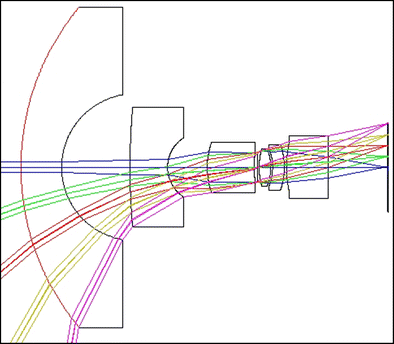
\includegraphics[scale=0.5]{pics/fisheye_scheme.png}                                                                                            %TODO: перерисовать схему?
        \caption{Системы кругового обзора}
        \label{pic:fyscheme}
    \end{center}
\end{figure}
    
Перед использованием снимков с подобных камер необходимо избавиться от искажений. Для осуществления этого необходима модель камеры - 
набор уравнений, который позволяет найти проекцию точки в мировых координатах на плоскость изображения. Стандартная для обычных камер 
модель камеры-обскуры хоть и способна учитывать радиальные искажения, не работает при таких больших углах зрения. В настоящий момент 
есть несколько распространённых моделей, аппроксимирующих реальные искажения подобных объективов. Модель Каналлы и Брандта \cite{opencv_model} 
реализована в OpenCV и предлагает 


\subsection{Обзор существующих систем стереозрения, использующих сверхширокоугольные изображения}

